\section{Atualidade de sistemas gerenciadores de agendamento}

Atualmente, soluções digitais para gerenciamento e agendamento de serviços já são personalizadas para o setor da beleza, e implementadas por meio de assinaturas. Algumas focam até mesmo na gestão de \emph{coworking}. Consequentemente, consolidaram-se funcionalidades padrão que são fundamentais para manter a competitividade no mercado. A Figura \ref{fig:modulos} ilustra os principais módulos embutidos em softwares e aplicativos disponíveis para espaços de beleza:

%inicio de figura
\begin{figure}[htb]
	\centering
	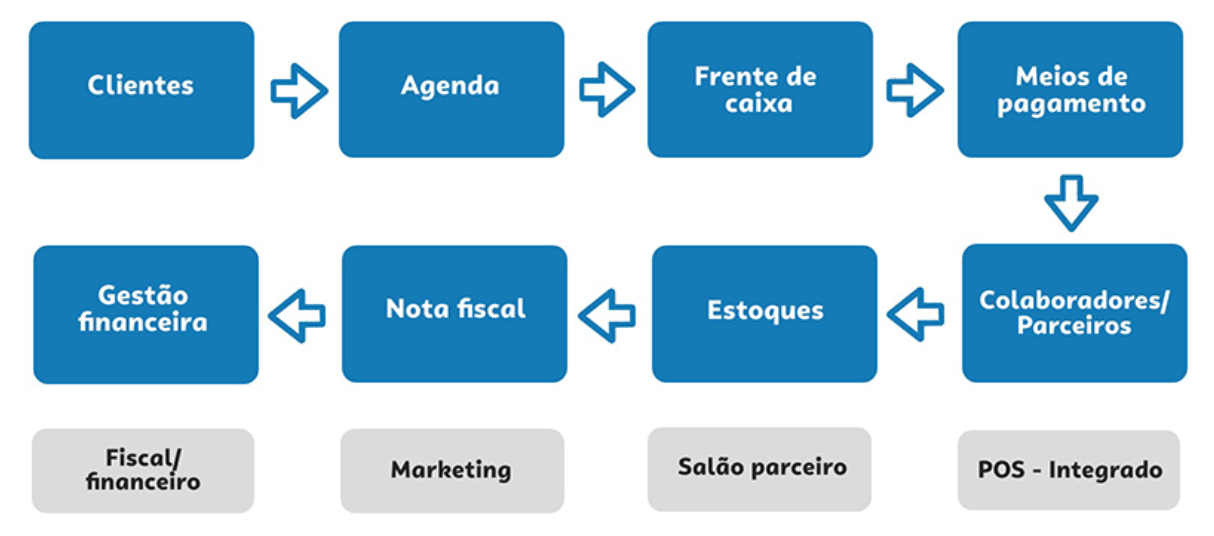
\includegraphics[width=0.7\textwidth]{cap02-Revisao_literatura/Images/modulos_basicos_sistema}
	\caption{módulos básicos em sistemas para salão de beleza}
	\label{fig:modulos}
	\fonte{\cite{Sebrae_beleza}}
\end{figure}


Pensando especificamente em \emph{coworkings} de beleza, surgem necessidades particulares:
\begin{itemize}
	\item Evitar sobreposições de horários em cadeiras, cabines ou equipamentos;
	\item Gerenciar a divisão de recursos (produtos ou aparelhos);
	\item Calcular automaticamente alugueis de estação ou comissões, com \emph{split} de pagamento entre o espaço e o profissional;
	\item Controlar acessos e permissões de cada perfil (administrador, profissional, cliente).
\end{itemize}

Embora algumas plataformas já ofereçam módulos de \emph{coworking}, muitas ainda exigem configurações e ajustes manuais para o cálculo de comissões e a alocação de recursos, o que gera retrabalho e eleva o risco de erros. Para enfrentar esses desafios, destacam-se hoje as seguintes tendências tecnológicas:
\begin{itemize}
	\item Aplicativos dedicados ao relacionamento independente entre profissionais e clientes para gestão de agenda;
	\item Pagamentos em tempo real;
	\item \emph{Dashboards} analíticos com indicadores de ocupação, performance individual e projeção de demanda.
\end{itemize}

No entanto, escolher uma solução digital para um \emph{coworking} de beleza vai além de automatizar processos e melhorar a gestão de serviços. Dada a rapidez do avanço tecnológico e a influência das informações na internet, o \emph{marketing} integrado e uma interface de usuário intuitiva passam a ser diferenciais decisivos. Um design previsível melhora a experiência, fideliza clientes e reduz o tempo de treinamento dos profissionais.
